\chapter{評価}
\par
行動情報と発話情報の両方を反映した心的状態の推定が有効であることを示すため,信念および欲求の推定において,MIoM SCAINと単一情報による心的状態推定システムUnimodal Inference of Mind SCAIN (UIoM SCAIN)を比較する.行動情報と発話情報には,本研究で作成したデータセットを利用する.


\section{実験設定}
\par
BToMによる信念および欲求の推定を評価するための実験を参考に,学生がアシストロボットとともに屋台で食事を買うシーンを想定する.図\ref{fig:ex_env1}に本実験における環境の一例を示す.
\begin{figure}[htbp]
  \begin{center}
    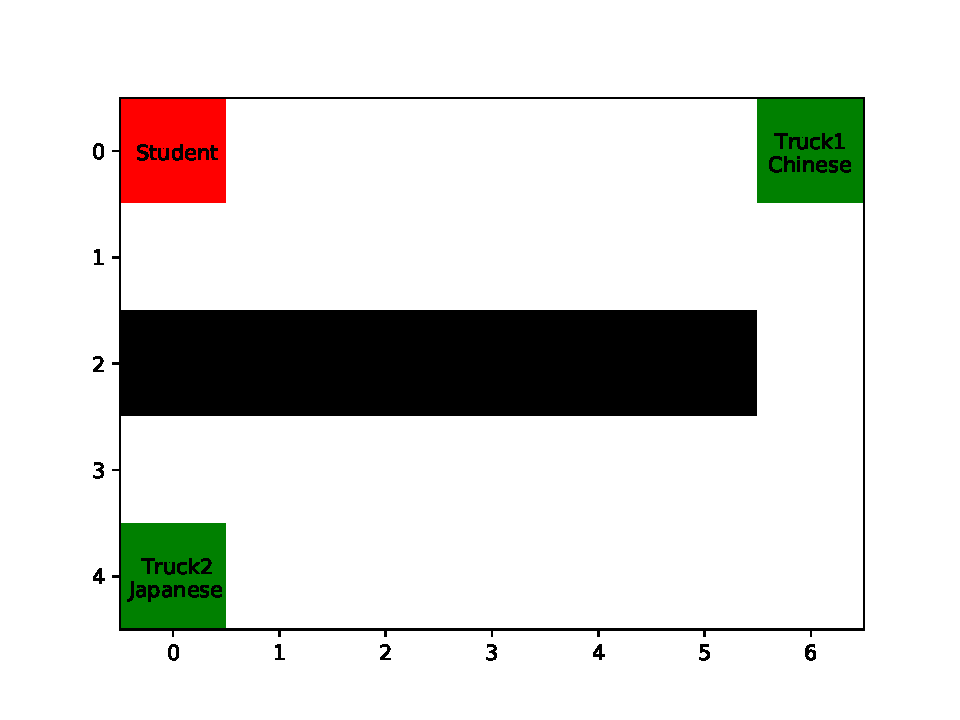
\includegraphics[scale=0.7]{./ex_env1.pdf}
    \caption{本実験における環境.図中の``Student''は学生,``Truck1''および``Truck2''は屋台を開くスペース,中央の黒色部分は壁を表す.}
    \label{fig:ex_env1}
  \end{center}
\end{figure}
7$\times$5マスで表現される環境中に壁とTruck1およびTruck2で表される屋台を開くスペースが存在し,それぞれのスペースに日本食の屋台,イタリア料理の屋台,中華料理の屋台のいずれかが出店する.環境中の学生は移動し,アシストロボットと対話をしながら食事を購入する屋台を決める状況を考える.学生は,日本食の屋台,イタリア料理の屋台,中華料理の屋台の3種類のうち2種類が出店することは知っているが,どの屋台が出店しているかは知らないため,環境中を移動しアシストロボットと対話しながら食事を買う屋台を選ぶ.学生の行動$a_t$は上,下,左,右の4方向への移動とし,発話$u_t$はアシストロボットから提示される食事に関する質問に対する学生の応答とする.信念$b_t$は,壁により観測できていない屋台に関してどの屋台が出店していると考えているか,欲求$d$は学生が3種類のそれぞれの屋台をどの程度好むかを表す.



\section{実験手順}

\par
本実験には,本研究で作成したデータセットを利用した.本データセットには,屋台の組み合わせを表す環境設定と,その環境設定で考えられる学生の行動,アシストロボットからの質問,学生の応答が含まれる.屋台の組み合わせは日本食の屋台,イタリア料理の屋台,中華料理の屋台の2つの組み合わせとする6通り,学生の行動は上,下,左,右の4方向への移動,アシストロボットからの質問は表\ref{tab:q_a}の左側に記載される4通り,学生の応答は表\ref{tab:q_a}の右側に記載される8通りである.
\begin{table}[htb]
  \begin{center}
  \caption{アシストロボットからの質問と学生の応答}
  \label{tab:q_a}
  \begin{tabular}{lll} \hline
    質問内容&\multicolumn{2}{l}{応答内容}\\\hline
    魚料理と野菜料理どちらを食べたいですか&fish&vegetable\\
    パスタと米ではどちらを食べたいですか&pasta&rice\\
    あっさりしたものと,こってりしたものどちらを食べたいですか&plain&oily\\
    辛いものと酸っぱいものではどちらを食べたいですか&spicy&sour\\\hline
  \end{tabular}
\end{center}
\end{table}
本実験では,一定時間パーティクルの尤度に大きな変化がない時およびTruck1を通り過ぎた時に質問を提示した.MIoM SCAINによって行動情報と発話情報の両方を推定に活用することが有効であることを評価するために,パーティクルフィルタを用い行動情報と発話情報の一方のみを基に心的状態を推定するシステムUnimodal Inference of Mind SCAIN (UIoM SCAIN)を定義した.


\par
図\ref{fig:interface}に示すインターフェスを用いて,30人の実験参加者に,本データセットで指定された環境設定と行動およびアシストロボットからの質問と学生の応答を提示し,環境中の学生の信念と欲求をそれぞれ7段階で推定させた.
\begin{figure}[htbp]
  \begin{center}
    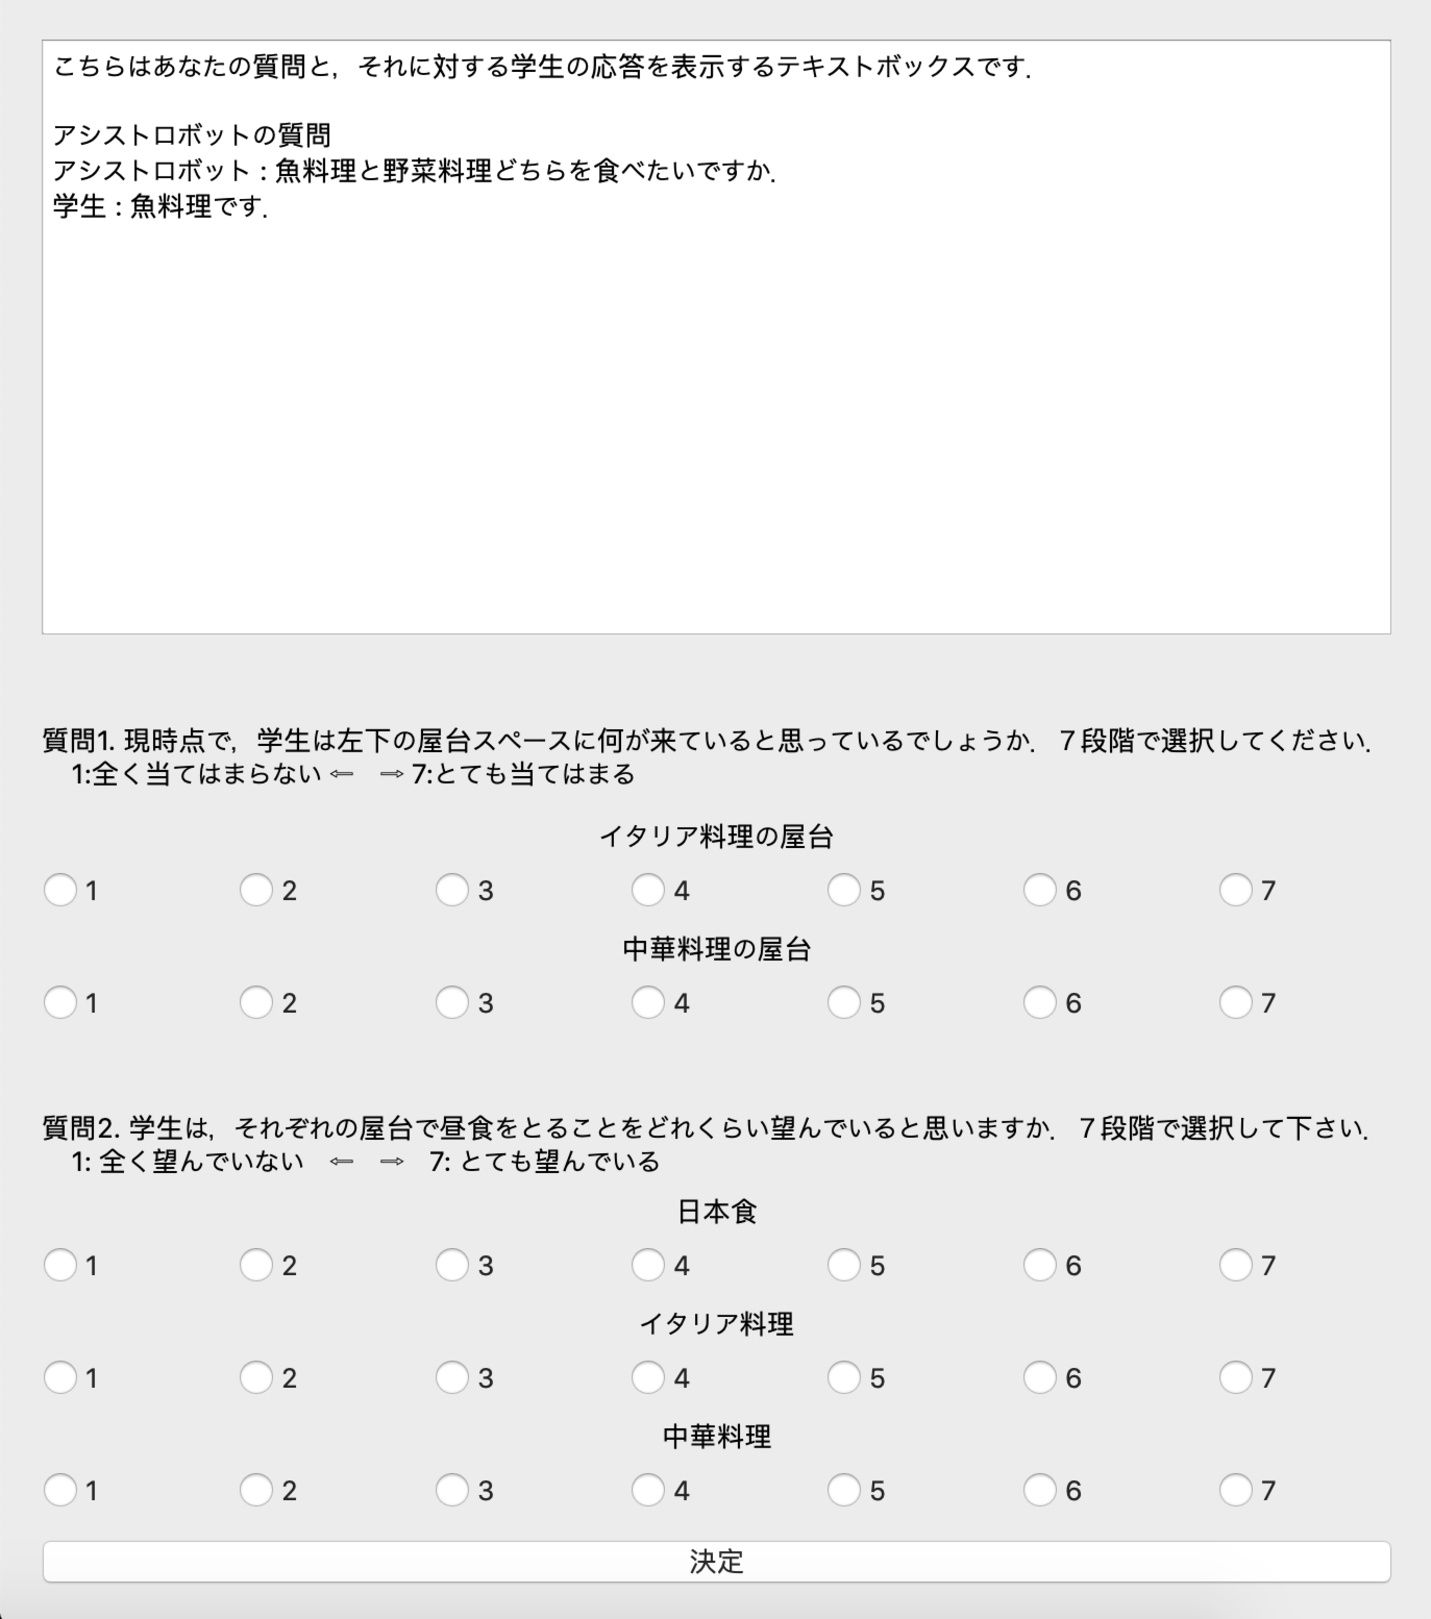
\includegraphics[scale=0.6]{./interface.pdf}
    \caption{本実験に使用したインターフェース}
    \label{fig:interface}
  \end{center}
\end{figure}
環境設定や行動の内容,アシストロボットからの質問,学生の応答に偏りがないように8つのデータを本データセットから選択し,それぞれの実験参加者に対して提示し,1つのデータに対して2回または3回推定をさせた.
また,MIoM SCAIN (action + utterance),行動情報のみを基に心的状態を推定するUIoM SCAIN (action),発話情報のみを基に心的状態を推定するUIoM SCAIN (utterance)の3つのシステムによって,環境中の学生の信念と欲求を推定し,推定結果を式(\ref{b_transform})および式(\ref{d_transform})により,7段階評価に変換した.
\begin{equation}
  \begin{split}
  \label{b_transform}
  b_t(\mathrm{Japanese})= \sum_{\substack{k\\b_t^k=\mathrm{Japanese}}} 7\cdot L^k\\
  b_t(\mathrm{Italian})=\sum_{\substack{k\\b_t^k=\mathrm{Italian}}} 7\cdot L^k\\
  b_t(\mathrm{Chinese})=\sum_{\substack{k\\b_t^k=\mathrm{Chinese}}} 7\cdot L^k\\
  \end{split}
\end{equation}

\begin{equation}
  \begin{split}
  \label{d_transform}
  d(\mathrm{Japanese})= \sum_{\substack{k\\d^k=\mathrm{Japanese}}} \frac{7}{3}\cdot L^k \cdot rank^k({\mathrm{Japanese}})\\
  d(\mathrm{Italian})= \sum_{\substack{k\\d^k=\mathrm{Italian}}} \frac{7}{3}\cdot L^k \cdot rank^k({\mathrm{Italian}})\\
  d(\mathrm{Chinese})= \sum_{\substack{k\\d^k=\mathrm{Chinese}}} \frac{7}{3}\cdot L^k \cdot rank^k({\mathrm{Chinese}})\\
  \end{split}
\end{equation}
ここで,$rank^k(\mathrm{food})$は,$k$番目のパーティクルにおける欲求$d_k$を基に$\mathrm{food}$をどの程度好むかを3段階で表した値である.式(\ref{b_transform})および式(\ref{d_transform})において,全てのパーティクルを考慮して計算を行うことで,各パーティクルの尤度に差がない場合に対応する.推定を行った全タイミングで,信念推定および欲求推定のそれぞれについて,実験参加者による推定結果とMIoM SCAINおよびUIoM SCAINによる推定結果を比較し,相関係数を算出した.UIoM SCAIN (action)およびUIoM SCAIN (utterance)の尤度は,それぞれ式(\ref{uiom_a}),式(\ref{uiom_u})で計算した.
\begin{equation}
  \begin{split}
  \label{uiom_a}
  L^k({\mathrm{action}})&= \sum_{b_{t-1}^k,o_t}P(b_t^k|b_{t-1}^k,o_t)\cdot P(o_t|s_t)\cdot P(s_t|s_{t-1},a_{t-1})\\
  &\hspace{3cm}\cdot P(a_{t-1}|b_{t-1}^k,d^k)\cdot P(b_{t-1}^k,d^k,s_{t-1},a_{t-2})
  \end{split}
\end{equation}

\begin{equation}
  \begin{split}
  \label{uiom_u}
  L^k({\mathrm{utterance}})&= \sum_{b_{t-1}^k,o_t}P(b_t^k|b_{t-1}^k,o_t)\cdot P(o_t|s_t)\cdot P(s_t|s_{t-1},a_{t-1})\\
  &\hspace{3cm}\cdot P(u_{t-1}|b_{t-1}^k,d^k)\cdot P(b_{t-1}^k,d^k,s_{t-1},u_{t-2})
  \end{split}
\end{equation}


\section{実験結果}

\par
表\ref{tab:cof}に,実験参加者による信念と欲求の推定結果とUIoM SCAIN (action), UIoM SCAIN (utterance)およびMIoM SCAINによる信念と欲求の推定結果との間の相関係数を示す.
\begin{table}[htb]
  \begin{center}
  \caption{人間による推定と推定モデルの相関}
  \label{tab:cof}
  \begin{tabular}{lcc} \hline
    \multirow{2}{*}{モデル}&\multicolumn{2}{c}{相関}\\\cline{2-3}
    & \hspace{10pt} 信念 \hspace{10pt} & \hspace{10pt} 欲求 \hspace{10pt} \\ \hline
    UIoM SCAIN (action)&0.124&0.419\\
    UIoM SCAIN (utterance)&0.216&0.494\\
    MIoM SCAIN (action + utterance)&\bf0.244&\bf0.549 \\\hline
  \end{tabular}
\end{center}
\end{table}

\par
表\ref{tab:cof}より,いずれの推定システムにおいても欲求推定の相関が信念推定の相関よりも強いことがわかった.

\par
また,信念と欲求の推定の両方において,行動情報と発話情報の両方を推定に活用するMIoM SCAINが行動情報のみを推定に活用するUIoM SCAIN (action)および発話情報のみを推定に活用するUIoM SCAIN (utterance)よりも強い相関を示すことがわかった.

\par
ここで,MIoM SCAINによる信念と欲求の推定の相関とUIoM SCAINによる信念と欲求の推定の相関との間に差があると言えるかを$z$検定\cite{alma9926301497204034}によって検定する.

\par
まず,MIoM SCAINとUIoM SCAIN (action)の信念推定における相関に差があるかを調べる.以下のように仮説を設定する.
\begin{displaymath}
  \begin{split}
  \label{z_a_b_p}
  \mathrm{帰無仮説:MIoM\; SCAINとUIoM\; SCAIN\; (action)の信念推定の相関に差がない}\\
  \mathrm{対立仮説:MIoM\; SCAINとUIoM\; SCAIN\; (action)の信念推定の相関に差がある}\\
  \end{split}
\end{displaymath}
また,データ数を考慮して統計検定量$T$は以下のように計算される.
\begin{displaymath}
  \begin{split}
  \label{z_a_b}
  T&=\sqrt{960-3}\left(\frac{1}{2}\ln{\frac{1-0.244}{1+0.244}-\frac{1}{2}\ln{\frac{1-0.124}{1+0.124}}}\right)\\
  &=3.85\\
  \end{split}
\end{displaymath}
$\alpha=0.05$で両側検定を行う.$z\left(\frac{\alpha}{2}\right)=1.96$であり,$T=3.85>1.96$なので,帰無仮説を棄却する.よって,MIoM SCAINとUIoM SCAIN (action)の信念推定における相関に差があると言える.

\par
次に,MIoM SCAINとUIoM SCAIN (utterance)の信念推定における相関に差があるかを調べる.以下のように仮説を設定する.
\begin{displaymath}
  \begin{split}
    \label{z_a_b}
    \mathrm{帰無仮説:MIoM\; SCAINとUIoM\; SCAIN\; (utterance)の信念推定の相関に差がない}\\
    \mathrm{対立仮説:MIoM\; SCAINとUIoM\; SCAIN\; (utterance)の信念推定の相関に差がある}\\
    \end{split}
\end{displaymath}
また,データ数を考慮して統計検定量$T$は以下のように計算される.
\begin{displaymath}
  \begin{split}
  \label{z_a_b}
  T&=\sqrt{960-3}\left(\frac{1}{2}\ln{\frac{1-0.244}{1+0.244}-\frac{1}{2}\ln{\frac{1-0.216}{1+0.216}}}\right)\\
  &=0.914\\
  \end{split}
\end{displaymath}
$\alpha=0.05$で両側検定を行う.$z\left(\frac{\alpha}{2}\right)=1.96$であり,$T=0.914<1.96$なので,帰無仮説を棄却しない.よって,MIoM SCAINとUIoM SCAIN (utterance)の信念推定における相関に差があるとは言えない.

\par
次に,MIoM SCAINとUIoM SCAIN (action)の欲求推定における相関に差があるかを調べる.以下のように仮説を設定する.
\begin{displaymath}
  \begin{split}
  \label{z_a_b}
  \mathrm{帰無仮説:MIoM\; SCAINとUIoM\; SCAIN\; (action)の欲求推定の相関に差がない}\\
  \mathrm{対立仮説:MIoM\; SCAINとUIoM\; SCAIN\; (action)の欲求推定の相関に差がある}\\
  \end{split}
\end{displaymath}
また,データ数を考慮して統計検定量$T$は以下のように計算される.
\begin{displaymath}
  \begin{split}
  \label{z_a_b}
  T&=\sqrt{1800-3}\left(\frac{1}{2}\ln{\frac{1-0.549}{1+0.549}-\frac{1}{2}\ln{\frac{1-0.419}{1+0.419}}}\right)\\
  &=7.23\\
  \end{split}
\end{displaymath}
$\alpha=0.05$で両側検定を行う.$z\left(\frac{\alpha}{2}\right)=1.96$であり,$T=7.23>1.96$なので,帰無仮説を棄却する.よって,MIoM SCAINとUIoM SCAIN (action)の欲求推定における相関に差があると言える.

\par
最後に,MIoM SCAINとUIoM SCAIN (utterance)の欲求推定における相関に差があるかを調べる.以下のように仮説を設定する.
\begin{displaymath}
  \begin{split}
  \label{z_a_b}
  \mathrm{帰無仮説:MIoM\; SCAINとUIoM\; SCAIN\; (utterance)の欲求推定の相関に差がない}\\
  \mathrm{対立仮説:MIoM\; SCAINとUIoM\; SCAIN\; (utterance)の欲求推定の相関に差がある}\\
  \end{split}
\end{displaymath}
また,データ数を考慮して統計検定量$T$は以下のように計算される.
\begin{displaymath}
  \begin{split}
  \label{z_a_b}
  T&=\sqrt{1800-3}\left(\frac{1}{2}\ln{\frac{1-0.549}{1+0.549}-\frac{1}{2}\ln{\frac{1-0.494}{1+0.494}}}\right)\\
  &=3.20\\
  \end{split}
\end{displaymath}
$\alpha=0.05$で両側検定を行う.$z\left(\frac{\alpha}{2}\right)=1.96$であり,$T=3.20>1.96$なので,帰無仮説を棄却する.よって,MIoM SCAINとUIoM SCAIN (utterance)の欲求推定における相関に差があると言える.
